
TDOA (Time Difference of Arrival) method, as one of the classic SSL (Sound Source Localization) method, performs excellently in environments with low noise and low reverberation. Its principle involves triangulating the position based on the time differences in the arrival of signals.

Assuming a system composed of two microphones located at coordinates \((x_1, y_1)\) and \((x_2, y_2)\), with the speed of sound in the current environment being \(c\). When a sound is emitted from the source and received by the two microphones, the TDOA value obtained is \(t_{12}\). Multiplying the TDOA value by \(c\) gives the distance difference between the sound source and the two microphones. Based on this, we can solve for the coordinates of the sound source:
\[
\sqrt{(x-x_{1})^{2}+(y-y_{1})^{2}}-\sqrt{(x-x_{2})^{2}+(y-y_{2})^{2}}=c*t_{1-2}
\]
Solving this equation, the result is a hyperbola representing all possible locations of the sound source under TDOA. By adding a third point, the intersection of two hyperbolas allows us to accurately determine the position of the sound source.\\
\begin{figure}[H]
    \centering
    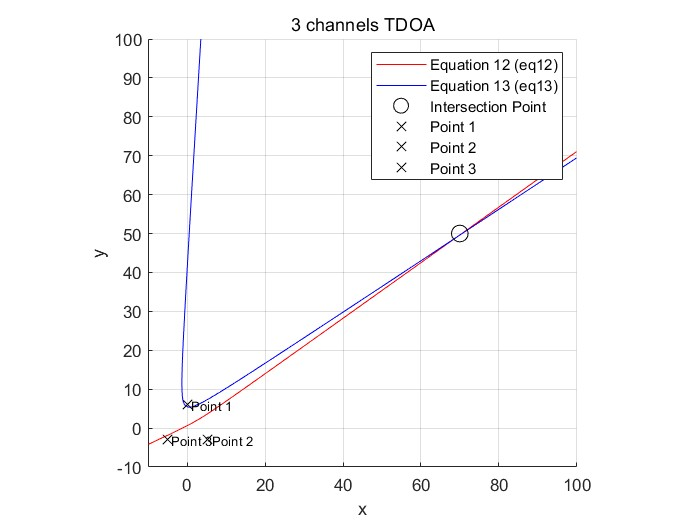
\includegraphics[width=0.7\linewidth]{figures/3_Channels.jpg}
    \caption{Enter Caption}
    \label{fig:enter-label}
\end{figure}
Generally, there are two ways to obtain TDOA values: 

The first method involves subtracting the time of arrival (TOA) at each receiver. The limitation of this approach is that acquiring TOA requires strict synchronization between the signal source and the receivers. Therefore, this method is not suitable for locating randomly occurring signal sources in an environment.

